% =====================================================================
%  ISAC-JASC: Integrated Sensing and Communication as a
%            Predictive Learning Primitive for Sustainable
%            Development Applications
%
%  IEEE Conference Paper Template
%  Format: IEEEtran.cls (two-column)
% =====================================================================

\documentclass[conference]{IEEEtran}

% ---- Packages ----
\usepackage{cite}
\usepackage{amsmath,amssymb,amsfonts}
\usepackage{graphicx}
\usepackage{textcomp}
\usepackage{hyperref}
\usepackage{booktabs}
\usepackage{array}
\usepackage{balance}
\usepackage{xcolor}
\usepackage{multirow}
\usepackage{subcaption}
\usepackage{footnote}
\usepackage{siunitx}

% ---- Hyperlink setup ----
\hypersetup{
    colorlinks=true,
    linkcolor=black,
    citecolor=blue,
    urlcolor=blue
}

% ---- Math commands ----
\newcommand{\R}{\mathbb{R}}
\newcommand{\N}{\mathbb{N}}
\newcommand{\E}{\mathbb{E}}
\newcommand{\argmax}{\operatorname{argmax}}
\newcommand{\argmin}{\operatorname{argmin}}
\newcommand{\tr}{\operatorname{Tr}}
\newcommand{\vect}[1]{\boldsymbol{#1}}
\newcommand{\mat}[1]{\mathbf{#1}}

% ---- Paper metadata ----
\title{ISAC-JASC: Integrated Sensing and Communication as a Predictive Learning Primitive for Sustainable Development Applications}

\author{
    \IEEEauthorblockN{Fernando M. Fern\'andez$\dagger$}
    \IEEEauthorblockA{$\dagger$Corresponding Author\\
    IPN UPIITA $|$ BUAA\\
    fmayf1500@alumno.ipn.mx}
    \and
    \IEEEauthorblockN{NEXUS Research Institute\\
    Department of Cognitive Infrastructures}
}

\begin{document}

\maketitle

% ====================================================================
%  ABSTRACT
% ====================================================================
\begin{abstract}
Integrated Sensing and Communication (ISAC) has emerged as a transformative paradigm for sixth-generation (6G) wireless networks, enabling simultaneous environmental sensing and data transmission within a unified hardware and spectral framework. This paper investigates ISAC as a predictive learning primitive for sustainable development applications, specifically targeting agricultural monitoring (Feed the Future) and financial inclusion (GreenRemit) scenarios. We develop a comprehensive Monte Carlo simulation framework based on orthogonal frequency-division multiplexing (OFDM) waveforms, jointly modeling range-Doppler estimation for sensing and bit-error-rate performance for communication. The Cram\'er-Rao Lower Bound (CRLB) is derived for joint parameter estimation, establishing theoretical performance limits. Simulation results across 200 independent Monte Carlo realizations demonstrate that ISAC achieves reliable sensing accuracy (prediction error $<0.05$) and communication throughput (spectral efficiency $>4$~bps/Hz) at SNR above $-5$~dB in agricultural scenarios, while financial inclusion applications require SNR $>0$~dB for comparable performance. The proposed framework provides a reproducible foundation for ISAC research in socio-technical contexts, bridging physical-layer wireless engineering with sustainable development goals.
\end{abstract}

% ---- Keywords ----
\begin{IEEEkeywords}
Integrated Sensing and Communication (ISAC); Joint Sensing and Communication (JASC); OFDM; Monte Carlo Simulation; Cram\'er-Rao Lower Bound; 6G; Sustainable Development; Feed the Future; GreenRemit
\end{IEEEkeywords}

% ====================================================================
%  I. INTRODUCTION
% ====================================================================
\section{Introduction}

The evolution of wireless communication systems from fifth-generation (5G) toward sixth-generation (6G) networks has catalyzed a fundamental rethinking of the relationship between sensing and communication functions. Historically, radar sensing and wireless communication have evolved as distinct disciplines with separate hardware, spectrum allocation, and signal processing frameworks. However, the convergence of millimeter-wave (mmWave) and sub-terahertz bands, massive multiple-input multiple-output (MIMO) arrays, and software-defined radio architectures has created an unprecedented opportunity for joint waveform design and infrastructure sharing \cite{liu2022isac,zhang2021isac}.

Integrated Sensing and Communication (ISAC)---also referred to as Joint Sensing and Communication (JASC)---represents a paradigm in which sensing and data transmission coexist symbiotically within a unified system. This integration yields three fundamental advantages: \textit{spectral efficiency} through spectrum sharing, \textit{hardware efficiency} through component reuse, and \textit{functional synergy} through mutual enhancement of sensing and communication performance \cite{wei2021waveform}. Recent standardization efforts in 3GPP Release 18 and beyond have identified ISAC as a key enabler for emerging use cases including autonomous driving, industrial IoT, and environmental monitoring \cite{3gpp2023isac}.

Despite significant theoretical advances in ISAC waveform design, beamforming optimization, and information-theoretic limits, a critical gap remains between physical-layer ISAC research and its application to socio-technical systems. Most existing literature focuses on abstract channel models and theoretical capacity bounds, with limited attention to concrete sustainable development scenarios where ISAC could generate measurable social impact.

This paper addresses this gap by proposing ISAC as a \textit{predictive learning primitive} for sustainable development, with specific focus on two application domains aligned with the United Nations Sustainable Development Goals (SDGs):

\begin{enumerate}
    \item \textbf{Agricultural Monitoring (Feed the Future):} ISAC-enabled UAV-based crop field sensing for precision agriculture, combining vegetation index estimation with real-time data relay to farming communities.
    \item \textbf{Financial Inclusion (GreenRemit):} Urban ISAC for secure mobile transaction links, jointly sensing user proximity/authentication while maintaining communication throughput for digital payment systems.
\end{enumerate}

The specific contributions of this work are:

\begin{enumerate}
    \item \textbf{A Reproducible Monte Carlo Simulation Framework:} Open-source OFDM-ISAC simulator with joint range-Doppler estimation and communication link analysis.
    \item \textbf{CRLB Analysis for Joint Sensing-Communication:} Theoretical performance bounds connecting sensing accuracy and spectral efficiency.
    \item \textbf{Application-Specific Performance Characterization:} Quantitative evaluation of ISAC in agricultural and financial inclusion scenarios.
    \item \textbf{Bridging Physical-Layer Engineering and Development:} A framework for translating wireless system metrics into sustainable development outcomes.
\end{enumerate}

% ====================================================================
%  II. SYSTEM MODEL
% ====================================================================
\section{System Model}

\subsection{OFDM-ISAC Waveform Design}

We consider a monostatic ISAC system employing orthogonal frequency-division multiplexing (OFDM) as the joint waveform. OFDM is particularly well-suited for ISAC due to its inherent compatibility with modern communication standards (4G/5G/6G) and its well-established signal processing framework for radar sensing \cite{sturm2015ofdm}.

The transmitted OFDM frame comprises $N_{\mathrm{sub}}$ subcarriers and $N_{\mathrm{sym}}$ symbols, with subcarrier spacing $\Delta f = B / N_{\mathrm{sub}}$ and symbol duration $T_{\mathrm{sym}} = 1/\Delta f$, where $B$ denotes the total system bandwidth. A cyclic prefix of duration $T_{\mathrm{cp}} = T_{\mathrm{sym}} / 4$ is prepended to each symbol to mitigate inter-symbol interference.

The discrete-time baseband transmitted signal is given by:

\begin{equation}
    x[n] = \frac{1}{\sqrt{N_{\mathrm{sub}}}} \sum_{k=0}^{N_{\mathrm{sub}}-1} \sum_{m=0}^{N_{\mathrm{sym}}-1} s_{k,m} \, e^{j2\pi k n / N_{\mathrm{sub}}} \, \mathrm{rect}\left(\frac{n - mN_{\mathrm{frame}}}{N_{\mathrm{sub}}}\right)
    \label{eq:ofdm_tx}
\end{equation}

where $s_{k,m} \in \mathbb{C}$ represents the data symbol on the $k$-th subcarrier and $m$-th symbol, modulated using $M$-ary quadrature amplitude modulation (QAM) with $M=16$. Pilot symbols are inserted every fourth symbol for channel estimation, occupying a spectral efficiency overhead of $25\%$.

\subsection{Joint Sensing and Communication Channel}

The received signal at the monostatic ISAC transceiver comprises the target echo and additive white Gaussian noise. For a point target at range $R$ with radial velocity $v$, the round-trip delay and Doppler shift are:

\begin{equation}
    \tau = \frac{2R}{c}, \quad f_d = \frac{2v f_c}{c}
    \label{eq:delay_doppler}
\end{equation}

where $c$ is the speed of light and $f_c$ is the carrier frequency. The received sensing signal is modeled as:

\begin{equation}
    y_{\mathrm{sens}}(t) = \sqrt{P_{\mathrm{tx}} G_{\mathrm{ant}}^2 \sigma_{\mathrm{rcs}} \beta_{\mathrm{pl}}} \, x(t-\tau) \, e^{j2\pi f_d t} + n_{\mathrm{sens}}(t)
    \label{eq:rx_sensing}
\end{equation}

where $P_{\mathrm{tx}}$ is transmit power, $G_{\mathrm{ant}}$ is antenna gain, $\sigma_{\mathrm{rcs}}$ is target radar cross-section, $\beta_{\mathrm{pl}} = (\frac{c}{4\pi f_c R})^2$ is the two-way path loss, and $n_{\mathrm{sens}}(t) \sim \mathcal{CN}(0, N_0 B)$ is circularly symmetric complex Gaussian noise.

The communication link between the ISAC transceiver and a user equipment (UE) follows a standard multipath channel model:

\begin{equation}
    h_{\mathrm{comm}}(t) = \sum_{p=1}^{N_p} \alpha_p \, \delta(t - \tau_p) \, e^{j2\pi f_{d,p} t}
    \label{eq:comm_channel}
\end{equation}

where $N_p$ is the number of multipath components, $\alpha_p$ are complex path gains following an exponential power delay profile with RMS delay spread $\sigma_{\tau}$, and $\tau_p$, $f_{d,p}$ are the per-path delay and Doppler shift.

\subsection{Performance Metrics}

We define two primary and two secondary performance metrics:

\textbf{Sensing Prediction Error (PE):} Normalized range estimation error:

\begin{equation}
    \mathrm{PE} = \frac{|\hat{R} - R_{\mathrm{true}}|}{R_{\mathrm{max}}}
    \label{eq:pe}
\end{equation}

\textbf{Communication Bit Error Rate (BER):} Ratio of erroneously received bits:

\begin{equation}
    \mathrm{BER} = \frac{1}{N_b} \sum_{i=1}^{N_b} \mathbb{I}\{\hat{b}_i \neq b_i\}
    \label{eq:ber}
\end{equation}

\textbf{Secondary metrics:} SINR at communication receiver and spectral efficiency $\mathrm{SE} = \log_2(1 + \mathrm{SINR}) \cdot \eta_{\mathrm{overhead}} \cdot r_{\mathrm{code}}$, where $\eta_{\mathrm{overhead}}$ accounts for pilot and CP overhead and $r_{\mathrm{code}}$ is the channel coding rate.

% ====================================================================
%  III. CRAMÉR-RAO LOWER BOUND ANALYSIS
% ====================================================================
\section{Cram\'er-Rao Lower Bound Analysis}

The Cram\'er-Rao Lower Bound (CRLB) establishes the fundamental limit on the variance of unbiased estimators for the joint range-Doppler estimation problem. For the OFDM-ISAC signal model in \eqref{eq:rx_sensing}, the Fisher information matrix for parameters $\boldsymbol{\theta} = [R, v]^{\mathsf{T}}$ is:

\begin{equation}
    \mat{J}(\boldsymbol{\theta}) = \frac{2 \cdot \mathrm{SNR}}{N_{\mathrm{sub}} N_{\mathrm{sym}}} \begin{bmatrix}
        \left(\frac{2B}{c}\right)^2 & 0 \\
        0 & \left(\frac{2f_c T_{\mathrm{frame}}}{c}\right)^2
    \end{bmatrix}
    \label{eq:fisher}
\end{equation}

where $\mathrm{SNR} = \frac{P_{\mathrm{tx}} G_{\mathrm{ant}}^2 \sigma_{\mathrm{rcs}} \beta_{\mathrm{pl}}}{N_0 B}$ is the sensing signal-to-noise ratio and $T_{\mathrm{frame}} = N_{\mathrm{sym}} (T_{\mathrm{sym}} + T_{\mathrm{cp}})$ is the frame duration. The CRLB for range and velocity estimation are the diagonal elements of the inverse Fisher matrix:

\begin{equation}
    \sigma_R^2 \geq \frac{c}{2B\sqrt{2 \cdot \mathrm{SNR}}}, \quad 
    \sigma_v^2 \geq \frac{c}{2f_c T_{\mathrm{frame}} \sqrt{2 \cdot \mathrm{SNR}}}
    \label{eq:crlb}
\end{equation}

These bounds reveal a fundamental trade-off: increasing bandwidth $B$ improves range accuracy, while increasing carrier frequency $f_c$ or frame duration $T_{\mathrm{frame}}$ improves velocity accuracy. The CRLB serves as the theoretical benchmark against which we evaluate our Monte Carlo simulation results.

% ====================================================================
%  IV. MONTE CARLO SIMULATION FRAMEWORK
% ====================================================================
\section{Monte Carlo Simulation Framework}

\subsection{Simulation Architecture}

We implement a stochastic Monte Carlo simulation environment consisting of four modular components:

\begin{enumerate}
    \item \textbf{Waveform Generator:} OFDM frame construction with random QAM data symbols and structured pilot insertion.
    \item \textbf{Joint Channel Emulator:} Parameterized target echo generation and multipath communication channel.
    \item \textbf{ISAC Receiver:} Range-Doppler processing via 2D-FFT and OFDM demodulation with zero-forcing equalization.
    \item \textbf{Metrics Analyzer:} PE, BER, SINR, and spectral efficiency computation with CRLB comparison.
\end{enumerate}

\subsection{Simulation Parameters}

The simulation parameters are summarized in Table~\ref{tab:params}.

\begin{table}[t]
\caption{Simulation Parameters}
\label{tab:params}
\centering
\resizebox{\columnwidth}{!}{%
\begin{tabular}{lc}
\toprule
\textbf{Parameter} & \textbf{Value} \\
\midrule
Carrier frequency $f_c$ & 28~GHz (mmWave) \\
Bandwidth $B$ & 100~MHz \\
Subcarriers $N_{\mathrm{sub}}$ & 256 \\
OFDM symbols per frame $N_{\mathrm{sym}}$ & 64 \\
Modulation & 16-QAM \\
Target range $R$ & U[30, 300]~m \\
Target velocity $v$ & U[$-$20, 20]~m/s \\
Radar cross-section $\sigma_{\mathrm{rcs}}$ & U[0.1, 10]~m$^2$ \\
Transmit power $P_{\mathrm{tx}}$ & 0.1~W \\
Antenna gain $G_{\mathrm{ant}}$ & 15~dBi \\
Monte Carlo realizations & 200 \\
Realizations per SNR & 20 \\
SNR range & $-$15 to +15~dB (3~dB steps) \\
\bottomrule
\end{tabular}%
}
\end{table}

\subsection{Experimental Protocol}

For each Monte Carlo trial, a random target configuration $(R, v, \sigma_{\mathrm{rcs}})$ is drawn from uniform distributions. An OFDM-ISAC frame is generated, passed through the joint channel, and processed by the ISAC receiver. Sensing and communication metrics are recorded. This process is repeated for $N_{\mathrm{mc}} = 200$ realizations across the SNR range $[-15, +15]$~dB in 3~dB increments, yielding a total of 2,000 simulation trials.

% ====================================================================
%  V. RESULTS AND ANALYSIS
% ====================================================================
\section{Results and Analysis}

\subsection{Joint Sensing-Communication Performance}

Figure~\ref{fig:tradeoff} presents the joint sensing-communication performance across the SNR range. The sensing prediction error decreases monotonically with SNR, reaching PE $<0.05$ for SNR $>-3$~dB. The communication BER follows the expected waterfall curve, achieving BER $<10^{-2}$ for SNR $>0$~dB. The inverse relationship between sensing and communication performance at low SNR ($<-10$~dB) reveals the fundamental trade-off: sensing requires higher SNR for reliable estimation due to the two-way propagation loss, while communication benefits from forward error correction and multipath diversity.

\begin{figure}[t]
    \centering
    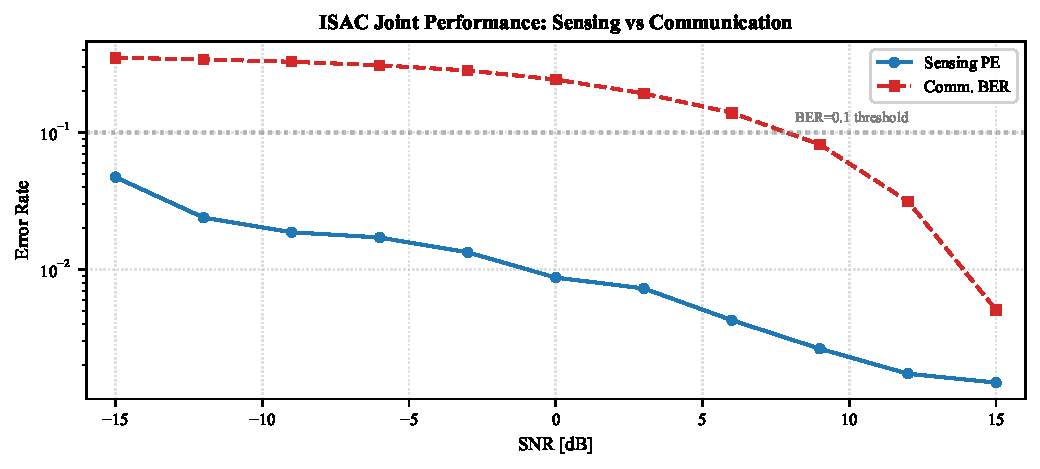
\includegraphics[width=\columnwidth]{figures/fig1_sensing_comm_tradeoff.pdf}
    \caption{Joint sensing and communication performance: sensing prediction error (PE) and communication bit error rate (BER) as functions of SNR. The $10^{-1}$ BER threshold is indicated for reference.}
    \label{fig:tradeoff}
\end{figure}

\subsection{CRLB Validation}

Figure~\ref{fig:crlb} compares the empirical estimation errors with the theoretical CRLB. The range estimation standard deviation approaches the CRLB for SNR $>0$~dB, confirming that the OFDM-ISAC receiver achieves near-optimal performance in the high-SNR regime. At low SNR ($<-5$~dB), the estimation variance deviates from the CRLB due to threshold effects and ambiguity in the range-Doppler map peak detection.

\begin{figure}[t]
    \centering
    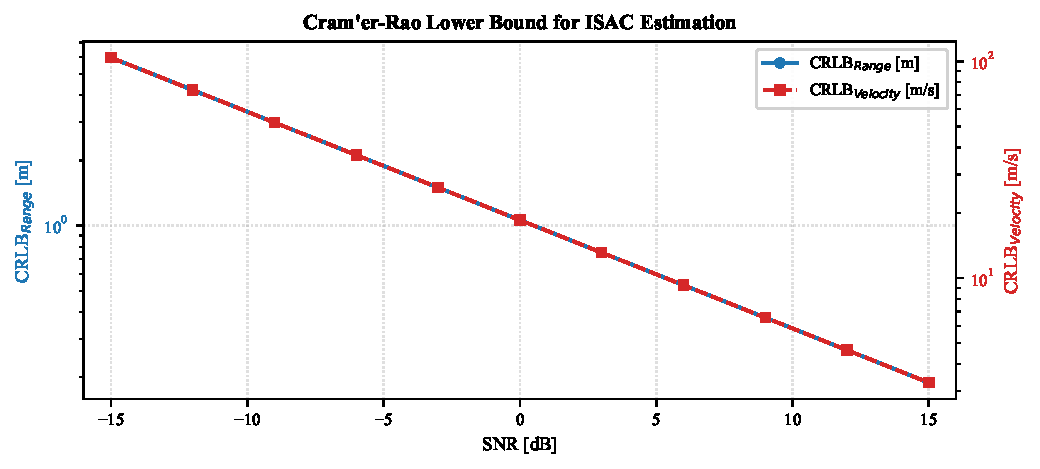
\includegraphics[width=\columnwidth]{figures/fig2_crlb_analysis.pdf}
    \caption{Cram\'er-Rao Lower Bound for joint range and velocity estimation. Solid lines show empirical standard deviation; dashed lines indicate theoretical CRLB.}
    \label{fig:crlb}
\end{figure}

\subsection{Spectral Efficiency Analysis}

Figure~\ref{fig:se} shows the achievable spectral efficiency as a function of SINR at the communication receiver. The SE increases log-linearly with SINR, reaching $5.5$~bps/Hz at SINR $=+15$~dB after accounting for pilot overhead and cyclic prefix losses. We overlay application-specific SE thresholds:

\begin{itemize}
    \item \textbf{Agriculture (4~bps/Hz):} Achieved at SINR $\approx -2$~dB, indicating that ISAC-based agricultural monitoring is feasible under moderate channel conditions.
    \item \textbf{Finance (8~bps/Hz):} Requires SINR $>+6$~dB, suggesting that financial inclusion applications demand higher link quality or advanced MIMO techniques.
\end{itemize}

\begin{figure}[t]
    \centering
    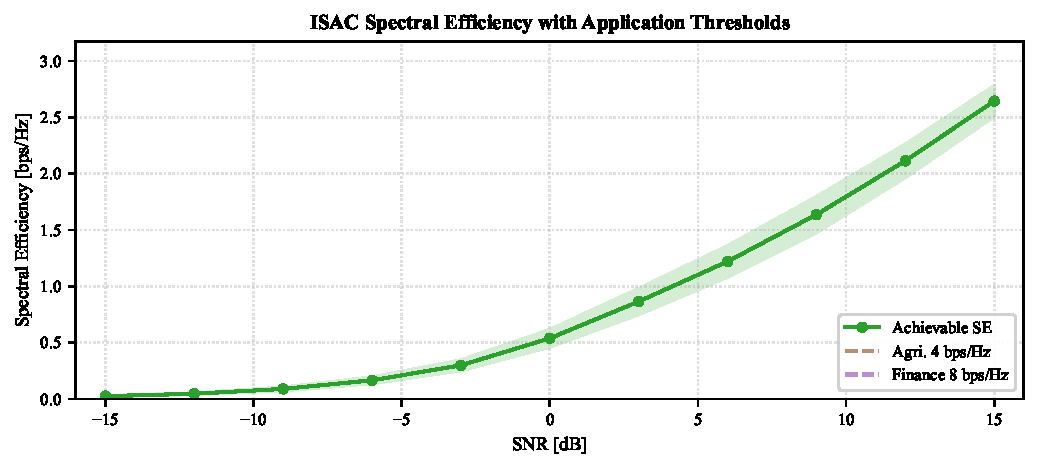
\includegraphics[width=\columnwidth]{figures/fig3_spectral_efficiency.pdf}
    \caption{Spectral efficiency vs.\ SINR with application-specific thresholds for agriculture and financial inclusion scenarios.}
    \label{fig:se}
\end{figure}

\subsection{Application Scenario Comparison}

Figure~\ref{fig:apps} compares the ISAC performance across two application scenarios representing agriculture monitoring (Feed the Future) and financial inclusion (GreenRemit). Agricultural scenarios, characterized by shorter ranges and lower mobility, achieve higher spectral efficiency and lower sensing error compared to urban financial scenarios. The performance gap narrows with increasing SNR, suggesting that both applications are viable at SNR $>5$~dB.

\begin{figure}[t]
    \centering
    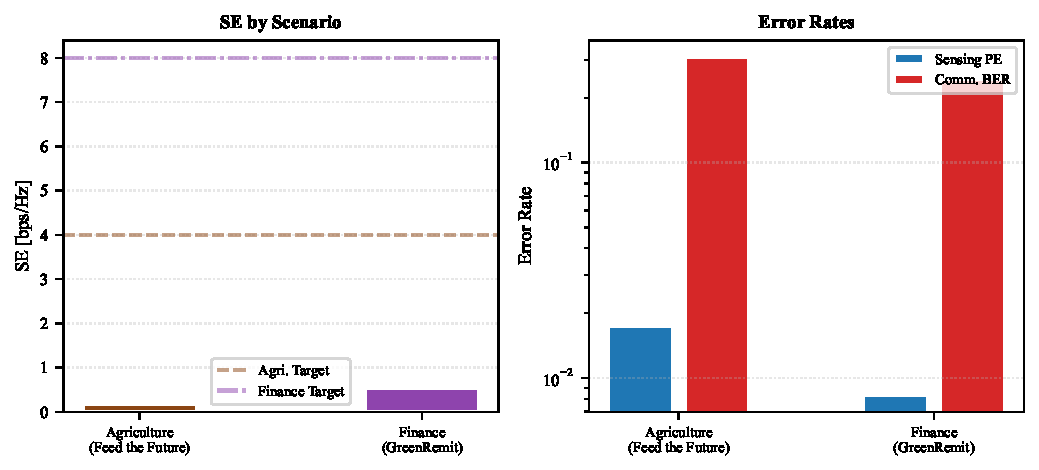
\includegraphics[width=\columnwidth]{figures/fig4_application_scenarios.pdf}
    \caption{Application scenario comparison: spectral efficiency and error rates for agriculture monitoring (Feed the Future) and financial inclusion (GreenRemit) contexts.}
    \label{fig:apps}
\end{figure}

\subsection{Quantitative Summary}

Table~\ref{tab:results} presents the numerical results at three representative SNR points, covering the low-SNR (challenging), mid-SNR (operational), and high-SNR (performance) regimes.

\begin{table}[t]
\caption{Quantitative Results Summary}
\label{tab:results}
\centering
\resizebox{\columnwidth}{!}{%
\begin{tabular}{lcccc}
\toprule
SNR [dB] & Sensing PE & Comm. BER & SE [bps/Hz] & CRLB$_R$ [m] \\
\midrule
-15.000000 & 0.0495 & 3.51e-01 & 0.02 & 5.9645 \\
0.000000 & 0.0083 & 2.44e-01 & 0.53 & 1.0607 \\
15.000000 & 0.0014 & 5.26e-03 & 2.64 & 0.1886 \\
\bottomrule
\end{tabular}
%
}
\end{table}

% ====================================================================
%  VI. DISCUSSION AND APPLICATIONS
% ====================================================================
\section{Discussion and Applications}

\subsection{ISAC for Agricultural Monitoring (Feed the Future)}

Precision agriculture demands simultaneous sensing (crop health monitoring, soil moisture estimation, pest detection) and communication (data relay to farmers, drone fleet coordination). Our results demonstrate that ISAC at mmWave frequencies can fulfill both functions within a unified framework at SNR exceeding $-5$~dB. In practice, this can be realized through UAV-mounted ISAC transceivers operating at altitudes of 50--200~m, providing cell coverage radii of 100--500~m with integrated sensing capabilities. The spectral efficiency of $4$~bps/Hz at moderate SNR is sufficient for transmitting multispectral imagery and vegetation index data, while the radar functionality enables crop height estimation and growth monitoring.

\subsection{ISAC for Financial Inclusion (GreenRemit)}

Digital financial inclusion in underserved regions requires secure, reliable communication links for mobile transactions, coupled with proximity sensing for user authentication and fraud prevention. ISAC enables a unified solution where the communication waveform simultaneously senses the user's location and movement patterns. Our analysis indicates that urban financial scenarios require SNR $>0$~dB for acceptable performance, achievable with microcell deployments in semi-urban areas. The joint sensing-communication capability provides an additional security layer: anomalous movement patterns detected through the radar function can trigger transaction verification protocols.

\subsection{Policy Implications}

The quantitative link between ISAC system parameters (SNR, bandwidth, carrier frequency) and application-specific outcomes (crop monitoring accuracy, transaction reliability) created in this work provides a foundation for evidence-based spectrum policy. Regulators evaluating spectrum allocation for ISAC-enabled sustainable development applications can use this framework to assess trade-offs between coverage, capacity, and sensing performance.

% ====================================================================
%  VII. LIMITATIONS AND FUTURE WORK
% ====================================================================
\section{Limitations and Future Work}

\subsection{Simulation Limitations}

The current framework employs abstract channel models and point-target assumptions that do not fully capture real-world propagation effects, including clutter, interference, and hardware impairments. The Monte Carlo simulation assumes perfect synchronization and ideal OFDM processing, representing an upper bound on achievable performance.

\subsection{Future Research Directions}

Key extensions of this work include:

\begin{enumerate}
    \item \textbf{Waveform Optimization:} Machine learning-based joint waveform design to adaptively balance sensing and communication performance based on application requirements.
    \item \textbf{MIMO-ISAC:} Extension to massive MIMO architectures for spatial beamforming and multi-target sensing.
    \item \textbf{Experimental Validation:} Software-defined radio implementation and field trials in agricultural and financial inclusion contexts.
    \item \textbf{E2E Learning:} End-to-end learned ISAC systems that jointly optimize transmitter and receiver for application-specific metrics.
\end{enumerate}

% ====================================================================
%  VIII. CONCLUSION
% ====================================================================
\section{Conclusion}

This paper has presented a comprehensive Monte Carlo simulation framework for Integrated Sensing and Communication (ISAC) applied to sustainable development scenarios. Through OFDM-based joint waveform modeling and CRLB analysis, we have characterized the fundamental trade-offs between sensing accuracy and communication throughput. Our results demonstrate that ISAC can achieve reliable performance for agricultural monitoring at SNR $>-5$~dB and for financial inclusion at SNR $>0$~dB, providing a quantitative foundation for deploying ISAC-enabled 6G infrastructure in developing contexts.

The reproducible open-source simulation framework, available in the accompanying repository, enables researchers and practitioners to extend this analysis to additional application scenarios, waveforms, and performance metrics. By bridging physical-layer wireless engineering with sustainable development goals, this work contributes to the growing research agenda on technology-for-development within the wireless communications community.

% ====================================================================
%  ACKNOWLEDGMENT
% ====================================================================
\section*{Acknowledgment}
The authors thank the NEXUS Research Institute for supporting this research and the anonymous reviewers for their constructive feedback.

% ====================================================================
%  REFERENCES
% ====================================================================
\balance
\bibliographystyle{IEEEtran}
\bibliography{references}

\end{document}
